\subsection{Authorization}
    \par
    The entire site is protected with the OAuth 2.0 token flow. Users login using a central authorization and receive a bearer token. This is send in the header of the request, as the user visits each microservice. As users persist their token locally between services this provides a seamless login experience.

\subsection{Internal Communications}
    \par
    To maintain compatibility between the various microservices a common messaging language was selected. Building on the groups experience writing web applications, we serialise messages into JSON and use REST APIs. These APIs can also be protected with the OAuth 2.0 authorization flow.

\subsubsection{Nginx}
    \begin{figure}[H]
        \centering
        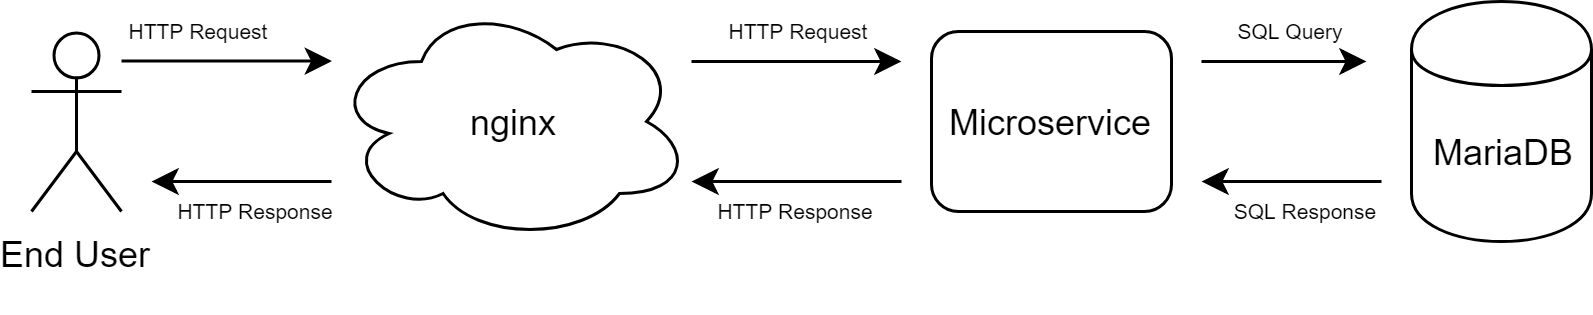
\includegraphics[width=\textwidth]{Images/nginx_proxy_flow.png}
        \caption{Traffic flow diagram showing an end user's browser connecting to the internet facing \textit{nginx} server, which then proxies requests through to the backend microservice}
    \end{figure}
    
    The Aber Fitness system architecture means that not exposed to the internet, but are instead available over an internal Docker network which allows containers to communicate with each other. In order to provide external access to the web servers of all of our microservices we have deployed nginx, an open-source and free web server which features highly customisable config files. Through the use of nginx's \lstinline{proxy\_pass} directive, we are able to take requests from end users and pass them through to the correct backend microservice based on the requested URI. \textbf{TODO: link figure above}
    

